\documentclass[a4paper]{article}
%
\usepackage{graphicx,tikz}
\usepackage{amsmath,amssymb}
\usepackage[hidelinks]{hyperref}
\usepackage{xcolor}
\usepackage{framed}
%
\renewenvironment{leftbar}[1][\hsize]
{%
    \def\FrameCommand
    {%
        {\color{red}\vrule width 2pt}%
        \hspace{0pt}%must no space.
        \fboxsep=2pt\colorbox{yellow}%
    }%
    \MakeFramed{\hsize#1\advance\hsize-\width\FrameRestore}%
}
{\endMakeFramed}
%
\graphicspath{{./figures/}}
%
\title{%
	\bfseries%
	{\large Numerical Techniques Practicum 1}\\[3ex]
	{\Large Getting started with LINUX and FORTRAN:}\\[1ex]
	{\Large Solving the oscillation equation.}
}
%
\author{Daan Degrauwe}
%
\addtolength\textwidth{4cm}
\addtolength\evensidemargin{-2cm}
\addtolength\oddsidemargin{-2cm}
\addtolength\voffset{-3cm}
\addtolength\textheight{5cm}
\setlength\parindent{0pt}
\setlength\parskip{5pt}
\setlength\parsep{5pt}
%
\usepackage{etoolbox}
\makeatletter
\preto{\@verbatim}{\topsep=2pt \partopsep=2pt }
%
\begin{document}
%
\maketitle
%
\par
Most NWP and climate models are Fortran codes working on Linux machines. For this reason, the exercises and projects for the Numerical Techniques course will be given in such an environment.
%
\par
Since not all students are familiar with Linux and/or Fortran, this first practicum is conceived as a step-by-step exercise, where both Linux basics and Fortran basics are dealt with.
%
\par
The goal is to write a Fortran program that calculates a numerical solution for the oscillation equation, as given by
%
\begin{equation*}
	\frac{d\psi}{dt}=i\kappa\psi
\end{equation*}
%
with initial condition $\psi_{t=0}=1$. The exact solution is given by $\psi(t)=\exp(i\kappa t)$.
%
\par
For this exercise, it is assumed that you work on the Linux server of UGENT (\texttt{helios}), and that you connect to it through the Athena platform.
%
\section{Different machines}
%
\par
During this exercise, three different machines should be distinguished:
%
\begin{itemize}
	\item the machine in front of you: PC in the PC-room, a laptop, a tablet or smartphone \ldots
	\item Athena, which in fact is a Windows machine that can be accessed via internet.
	\item \texttt{helios}, which is a Linux server of UGENT.
\end{itemize}
%
Note that Athena and \texttt{helios} are \emph{remote} machines: they may not even be in the same building as where you are.
%
\par
The reason why several machines are needed is that each operating system has its strong and weak points. While a graphical user-interface like Windows is most convenient for user interaction and visualization, Linux is more convenient for calculations and repetitive tasks. The intermediate layer of Athena is used to ensure that everyone works in the same environment.
%
\subsection{Athena}
%
\par
To log in on Athena, open a web browser, and go to \texttt{https://athena.ugent.be}. Log in with your UGENT user and password. You should then see a page like this:
%
\begin{center}
	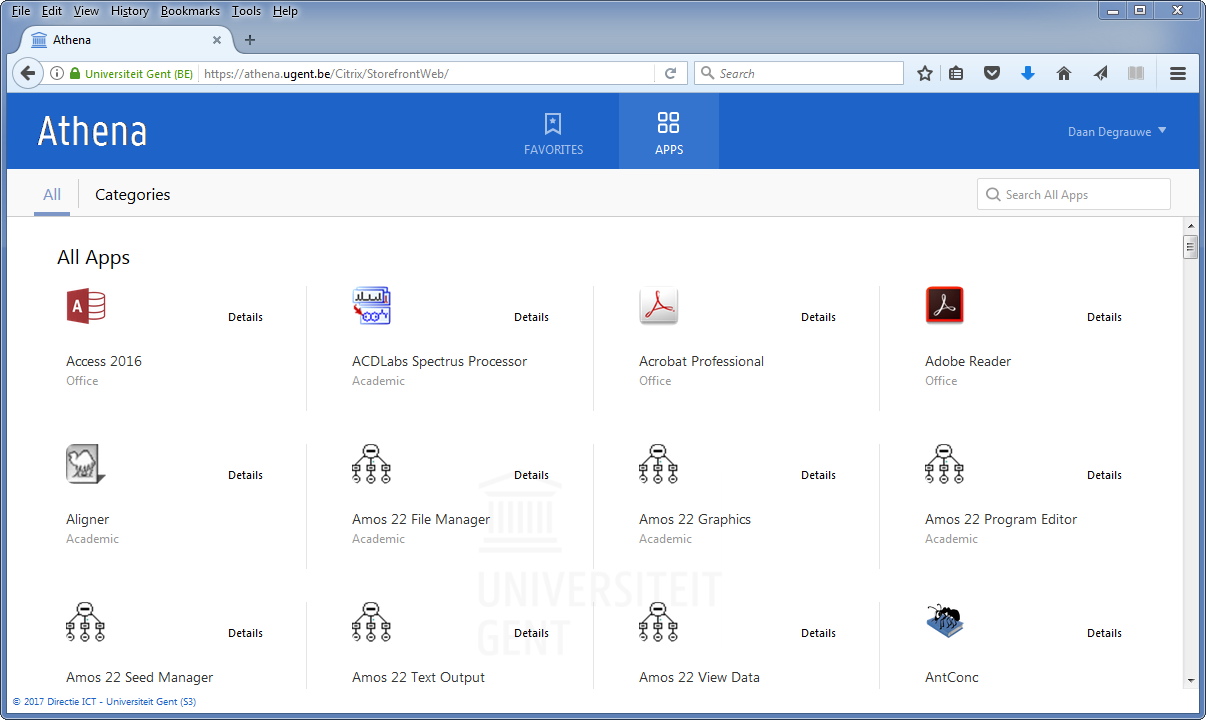
\includegraphics[scale=.45]{athena2.png}
\end{center}
%
\subsection{helios}
%
\par
First, an account should be created on \texttt{helios}. To do so, go to\\ \verb+https://helpdesk.ugent.be/account/en/helios.php+, and follow the guidelines there.
%
\par
Next, from Athena, open the program PuTTY. It should give you a window like this:
%
\begin{center}
	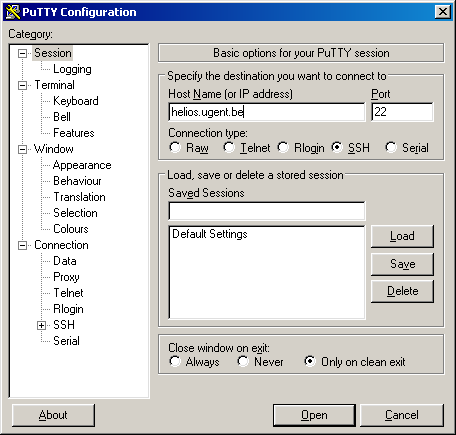
\includegraphics[scale=.45]{putty1.png}
\end{center}
%
\par
Set the Host Name to \emph{helios.ugent.be}. Optionally, give the session a name and save it for future use. Then hit the ``Open'' button. This will open a window where you are asked to enter your helios account and password.
%
\begin{center}
	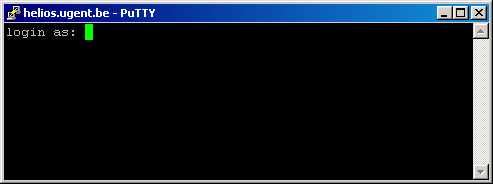
\includegraphics[scale=.45]{putty2.png}
\end{center}
%
\par
After entering account name and password (note the password doesn't appear when typed, not even as ******), the following screen appears
%
\begin{center}
	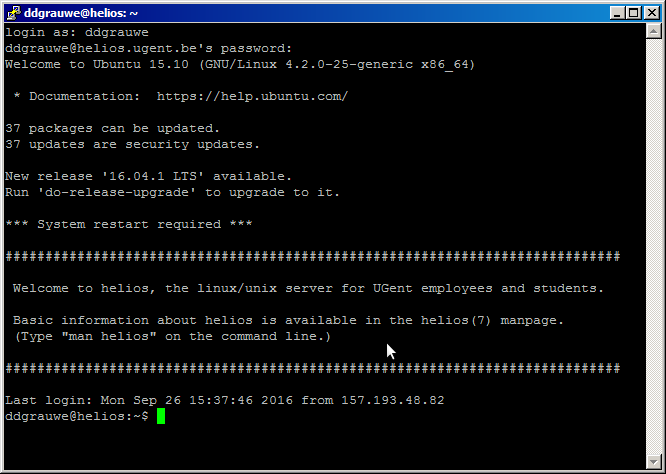
\includegraphics[scale=.45]{putty3.png}
\end{center}
%
\par
Congratulations, you are now connected to a Linux machine. What you see is called the \emph{command line}. In Linux, almost everything you do is done by typing commands on the command line. For instance, try to execute the following command:
%
\begin{verbatim}
   $   date
\end{verbatim}
%
where the \texttt{\$} denotes that the command should be typed in the command line. The \texttt{\$} should not be typed itself! Hitting \texttt{ENTER} after this command prints the current date on the screen.
%
\par
Note: Linux is case-sensitive. This means that typing \verb+DATE+ or \verb+Date+ will not work.
%
\par
The Linux commands that are needed for this lesson will be explained during the course of the exercise. Appendix~\ref{sec:linux_commands} gives an overview of some of the most common Linux commands. At this point, you get three tricks for free:
%
\begin{itemize}
	\item Linux stores a history of commands you entered. To repeat a previous command, hit the \texttt{UP} arrow.
	\item Hitting the \texttt{TAB} key autocompletes. For example, if you type \texttt{dat}, and then hit \texttt{TAB}, it will autocomplete to \texttt{date}. This also works for files and directories. If multiple options exist for autocompletion, you can hit \texttt{TAB} twice, to see the options. For instance, if you type \texttt{da}, and then hit \texttt{TAB} twice, you should see that \texttt{date} and \texttt{dash} are possible commands.
	\item You can copy/paste text in the PuTTY window by selecting the text with the left mouse button, and pasting it with the right mouse button.
\end{itemize}
%
\par
When working on a Linux command line, it is important to note that one works in a specific directory. Normally, this directory is visible before the \texttt{\$} symbol. You can also use the \verb+pwd+ command to print the working directory.
%
\subsection{Data transfer between Athena and \texttt{helios}}
%
\par
As explained before, Athena and \texttt{helios} are actually two different machines. Luckily, it is possible to mount the same drive (the so-called ``H-drive'') on the two systems. This makes transfering data between both machines much easier.
%
\par
To mount the H-drive on \texttt{helios}, execute the following command:
%
\begin{verbatim}
   $   newns  -i
\end{verbatim}
%
After providing your password, you can access the H-drive with
%
\begin{verbatim}
   $   cd /files/${USER}/home/
\end{verbatim}
%
Note: these two commands should be executed everytime you log in on \texttt{helios}.
%
\subsection{Creating and modifying a text file}
%
\par
Creating and modifying text files is very important for the rest of this exercise (and the remainder of the course). Make sure to go through this section meticulously.
%
\subsubsection{File creation on \texttt{helios}}
%
\par
To create a file on the H-drive, execute the following commands:
%
\begin{verbatim}
   $   mkdir /files/${USER}/home/numtech
   $   cd /files/${USER}/home/numtech
   $   touch test.txt
\end{verbatim}
%
Some explanation:
%
\begin{itemize}
	\item \texttt{mkdir} creates a new directory
	\item with \texttt{cd}, you go to this directory
	\item \texttt{touch} creates a (empty) file
\end{itemize}
%
To check if the file was indeed created, run the following command:
%
\begin{verbatim}
   $   ls
\end{verbatim}
%
which gives a listing of the files in the current directory.
%
\subsubsection{Modification on Athena\label{sec:txtmodif}}
%
\par
Now, we will modify this file using a text editor on Athena. 
%
\begin{enumerate}
	\item open the {Notepad++} editor in Athena
	\item inside {Notepad++}, open the file \verb+H:\numtech\test.txt+ (which is still empty for now).
	\item put some text in the file (e.g. ``Hello World!'').
	\item \textbf{Important}: make sure to set the end-of-line convention correctly for this file:\\ Edit$\rightarrow$EOL Conversion$\rightarrow$Unix/OSX Format. It's best to do this always for files you will use in Linux.
	\item Save the file
\end{enumerate}
%
\subsubsection{Review on \texttt{helios}}
%
\par
To check if everything went well, run the following command on \texttt{helios}:
%
\begin{verbatim}
   $   cat test.txt
\end{verbatim}
%
which should show you the text you entered in {Notepad++}.
%
\section{My first Fortran program}
%
\subsection{The Fortran code}
%
\par
First, create a directory for this program on the H-drive, and create an empty file \texttt{osceq.F90}:
%
\begin{verbatim}
   $   mkdir /files/${USER}/home/numtech/osceq
   $   cd /files/${USER}/home/numtech/osceq/
   $   touch osceq.F90
\end{verbatim}
%
\par
Open this file in {Notepad++}, and put the following Fortran code inside:
%
{\vspace{10pt}\hrule\small\vspace*{-2pt}\begin{verbatim}
	  PROGRAM OSCEQ
	  ! a program to solve the oscillation equation
	  
	  WRITE (*,*) "Welcome to the Oscillation Equation Solver."
	  
	  END PROGRAM OSCEQ
\end{verbatim}\hrule\vspace{5pt}}
%
Some explanations:
%
\begin{itemize}
	\item \verb+PROGRAM+ and \verb+END PROGRAM+ statements indicate the start and end of our program
	\item Text after a \verb+!+ denotes a comment. Use comments abundantly to make notes on the code.
	\item The \verb+WRITE+ statement is used to print text on the screen, or to write text to a file (see later). The argument \verb+(*,*)+ means that writing should be done to screen, in default formatting.
	\item Fortran is not case sensitive. This means it doesn't matter whether you write \verb+PROGRAM+ or \verb+program+ or \verb+PrOgRaM+.
\end{itemize}
%
\subsection{Compiling\label{sec:compile}}
%
\par
Before being able to execute Fortran code, it must be \emph{compiled}. This is the process of transforming a code that's readable to humans (Fortran) into a code that's readable to computers (executable files). For this, we use a \emph{compiler}.
%
\par
Compilation is quite easy (as long as your code doesn't contain any mistakes). On \texttt{helios}, we will use the \texttt{gfortran} compiler. To convert the Fortran code into an executable program, type the following in the command line:
%
\begin{verbatim}
	  $   gfortran osceq.F90 -o osceq
\end{verbatim}
%
This command tells \verb+gfortran+ the following: take the file \verb+osceq.F90+, convert it to an executable program, and put the result in the file \verb+osceq+.
%
\par
If all goes well, you should now have two files in the directory: \verb+osceq.F90+ and \verb+osceq+. You can check this with the Linux \verb+ls+ command. If you don't see the file \verb+osceq+, the compilation failed, most probably due to a coding mistake in the Fortran file. If you encounter errors during the compilation, try to understand what went wrong. Always look at the first error (later errors may be consequence of the first error). Ask for help if necessary: don't lose too much time on practicalities. You can use comments to indicate where you made a mistake in your program, in order to avoid such mistakes in the future.
%
\par
\textbf{Remark}: make sure to recompile the program after every modification of the Fortran file!
%
\subsection{Running\label{sec:run}}
%
\par
To execute the program, type the following on the command line:
%
\begin{verbatim}
   $   ./osceq
\end{verbatim}
%
This will print some text to screen.
%
\subsection{Automating tasks with Linux scripts}
%
\par
You may have noticed that recompiling and running often go together. It is therefore useful to create a Linux script that automates these two tasks. First create a file \texttt{run.sh}:
%
\begin{verbatim}
   $   touch run.sh
   $   chmod +x run.sh
\end{verbatim}
%
Where the \verb+chmod+ command marks the file as an executable script.
%
\par
Next, open this file in {Notepad++}, and put the following text in it:
%
{\vspace{10pt}\hrule\small\vspace*{-2pt}\begin{verbatim}
    # Script to compile and run the oscillation equation program
    
    # remove executable file
    rm osceq
    
    # Compile
    echo "Compiling"
    gfortran -o osceq osceq.F90
    
    # Run
    echo "Running"
    ./osceq
\end{verbatim}\hrule\vspace{5pt}}
%
%
Some explanations:
%
\begin{itemize}
	\item Comments in Linux scripts are indicated by a \verb+#+.
	\item The \verb+rm+ command removes the existing executable.
	\item The \verb+echo+ command prints text to the screen.
\end{itemize}
%
Also, remember to set the end-of-line convention to Unix/OSX, as explained under~\ref{sec:txtmodif}.
%
\par
Running the script is done with
%
\begin{verbatim}
   $   ./run.sh
\end{verbatim}
%
\section{Defining and using variables in Fortran}
%
\par
Let us now introduce some variables in our Fortran program. However, before making further modifications, it is good practice to take a copy of the current directory:
%
\begin{verbatim}
   $   cd ..
   $   cp -r osceq/ osceq_v1
   $   cd osceq/
\end{verbatim}
%
With the first command, we move one directory up (so to \verb+/files/${USER}/home/numtech/+). The \verb+cp+ command takes a copy; to copy directories, the additional argument \verb+-r+ is required.
%
\par
Now we have stored a backup, we can proceed with modifying the source code. In {Notepad++}, change the file \texttt{osceq.F90} as follows:
%
{\vspace{10pt}\hrule\small\vspace*{-2pt}\begin{verbatim}
	  PROGRAM OSCEQ
	  ! a program to solve the oscillation equation
	  
	  IMPLICIT NONE       ! safety to make sure all variables are declared
	  
	  ! declarations
	  REAL    :: KAPPA    ! parameter kappa in the oscillation equation (frequency)
	  REAL    :: DT       ! timestep
	  INTEGER :: NT       ! number of timesteps
	  COMPLEX :: PSI0     ! initial condition

	  WRITE (*,*) "Welcome to the Oscillation Equation Solver."
	  
	  ! initialize parameters
	  KAPPA = 0.5
	  DT    = 1.0
	  NT    = 20
	  PSI0  = COMPLEX(1.0,0.0)      ! complex number 1.0 + 0.0 * i
	  
	  WRITE (*,*) 'Total integration time = ',NT*DT
	  WRITE (*,*) 'Courant number = ',KAPPA*DT
	  
	  END PROGRAM OSCEQ
\end{verbatim}\hrule\vspace{5pt}}
%
Compile and run this program by running the \verb+run.sh+ script.
%
\par
The program contains the following new ingredients:
%
\begin{itemize}
	\item The statement \verb+IMPLICIT NONE+ is a safety. It's good practice to put it in all your Fortran programs. It means that all variables should be declared explicitly.
	\item The statements \verb+REAL+, \verb+INTEGER+ and \verb+COMPLEX+ are used to \emph{declare} variables. Declaration is where you tell the compiler what kind a certain variable is. Besides REAL, INTEGER and COMPLEX, Fortran also knows CHARACTER and LOGICAL types.
	\item The variables are \emph{assigned} their values with the \verb+=+ operator.
	\item The variables can then be used in calculations as shown in the \verb+WRITE+ statements
\end{itemize}
%
\par
It is important to be aware of the types of variables. For instance, the numbers \verb+2+ and \verb+5+ are of type \verb+INTEGER+. This means that \verb+5/2+ will take value \verb+2+, because dividing two variables of type \verb+INTEGER+ results in another \verb+INTEGER+! To correctly perform divisions, make sure that one of the numbers is of type \verb+REAL+. For example, \verb+5.0/2+ will give you the desired \verb+2.5+.
%
\par
It should be mentioned that the organization of a Fortran program is quite strict: \emph{all} declarations should come before the executable statements. If you want to introduce a new variable, it should be declared at the beginning of the program, even if you only use it somewhere at the end.
%
\section{Loops}
%
\par
Now we get to the actual purpose of our program: the time integration. We will do this with the forward scheme, for which
%
\begin{equation*}
	\phi^{n+1}=(1+i\kappa\Delta t)\phi^n
\end{equation*}
%
\par
The time integration is a repetitive task: given the solution at the current timestep ($\phi^n$), the solution at the next timestep ($\phi^{n+1}$) is calculated. A repetitive task is implemented in Fortran with a \verb+DO+-loop.
%
\par
First, store a copy of your program with
%
\begin{verbatim}
   $   cd ..
   $   cp -r osceq/ osceq_v2
   $   cd osceq/
\end{verbatim}
%
\par
Then, modify the file \verb+osceq.F90+ as follows:
%
{\vspace{10pt}\hrule\small\vspace*{-2pt}\begin{verbatim}
	  PROGRAM OSCEQ
	  ! a program to solve the oscillation equation

	  IMPLICIT NONE       ! safety to make sure all variables are declared

	  ! declarations
	  REAL    :: KAPPA    ! parameter kappa in the oscillation equation (frequency)
	  REAL    :: DT       ! timestep
	  INTEGER :: NT       ! number of timesteps
	  INTEGER :: IT       ! current timestep
	  COMPLEX :: PSI0     ! initial condition
	  COMPLEX :: PSI, PHI ! exact and numerical time-solution
	  COMPLEX :: II       ! imaginary unit

	  ! initialize parameters
	  KAPPA = 0.5
	  DT    = 1.0
	  NT    = 20
	  PSI0  = COMPLEX(1.,0.)
	  II    = COMPLEX(0.,1.)

	  ! set initial conditions
	  IT=0
	  PSI=PSI0
	  PHI=PSI0
	  ! show values at zero'th timestep
	  WRITE (*,*) 't = ',IT*DT,'; PSI = ',REAL(PSI),'; PHI = ',REAL(PHI)

	  ! start loop over timesteps
	  DO IT = 1,NT

	    ! exact solution
	    PSI = EXP(II*KAPPA*DT)*PSI

	    ! numerical solution: forward scheme
	    PHI = (1+II*KAPPA*DT)*PHI

	    ! show values at current timestep
	    WRITE (*,*) 't = ',IT*DT,'; PSI = ',REAL(PSI),'; PHI = ',REAL(PHI)

	  ENDDO

	  END PROGRAM OSCEQ
\end{verbatim}\hrule\vspace{5pt}}
%
\par
New ingredients are:
%
\begin{itemize}
	\item The functions \verb+REAL()+ and \verb+EXP()+, which respectively take the real part of a complex number, and the exponential function
	\item The statements \verb+DO IT=1,NT+ and \verb+ENDDO+ denoting the start and end of a \emph{loop}. The enumerator \verb+IT+ takes the initial value of 1, and augments every timestep by 1, until it gets larger than \verb+NT+.
\end{itemize}
%
\par
When running the program, it should become clear that the forward scheme is unstable.
%
\section{Conditions}
%
\par
Conditional branching in Fortran is done with the \verb+IF+ statement. For instance, we could introduce the following piece of code to check for an unstable scheme:
%
{\vspace{10pt}\hrule\small\vspace*{-2pt}\begin{verbatim}
	  PROGRAM OSCEQ
	  ! a program to solve the oscillation equation
	  
	  ... (see previous version of the program)
	  
	  ! start loop over timesteps
	  DO IT = 1,NT
	  
	    ! numerical solution: forward scheme
	    PHI = (1+II*KAPPA*DT)*PHI
	    
	    ! warning if unstable
	    IF ( ABS(PHI) > 10.0 ) THEN
	      WRITE (*,*) 'WARNING: unstable behaviour detected'
	    ENDIF
	  
	  ENDDO
	  
	  END PROGRAM OSCEQ
\end{verbatim}\hrule\vspace{5pt}}
%
\par
When running long enough (\verb+NT+$\geq21$), you should see a warning in the output.
%
\par
More advanced conditions are achieved with \verb+.AND.+, \verb+.OR.+ and \verb+.NOT.+. If you want to execute some code when the condition is \emph{not} fulfilled, use the \verb+ELSE+ statement.
%
\section{Arrays}
%
\par
Arrays are collections of numbers. In this program, they allow to store the solution for the full time-range. Consider the following program:
%
{\vspace{10pt}\hrule\small\vspace*{-2pt}\begin{verbatim}
	  PROGRAM OSCEQ
	  ! a program to solve the oscillation equation

	  IMPLICIT NONE       ! safety to make sure all variables are declared

	  ! declarations
	  REAL    :: KAPPA    ! parameter kappa in the oscillation equation (frequency)
	  REAL    :: DT       ! timestep
	  INTEGER :: NT       ! number of timesteps
	  INTEGER :: IT       ! current timestep
	  COMPLEX :: PSI0     ! initial condition
	  COMPLEX :: II       ! imaginary unit
	  COMPLEX, ALLOCATABLE :: PSI(:), PHI(:) ! arrays of exact and numerical solution

	  ! initialize parameters
	  KAPPA = 0.5
	  DT    = 1.0
	  NT    = 100
	  PSI0  = COMPLEX(1.,0.)
	  II    = COMPLEX(0.,1.)

	  ! allocate memory for arrays
	  ALLOCATE(PSI(0:NT),PHI(0:NT))

	  ! set initial conditions
	  IT=0
	  PSI(IT)=PSI0
	  PHI(IT)=PSI0

	  ! start loop over timesteps
	  DO IT = 1,NT
	  	
	  	! exact solution
	  	PSI(IT) = EXP(II*KAPPA*DT)*PSI(IT-1)
	  	
	  	! numerical solution: forward scheme
	  	PHI(IT) = (1+II*KAPPA*DT)*PHI(IT-1)
	  	
	  ENDDO

	  ! show values
	  WRITE (*,*) 'PSI = ',REAL(PSI)
	  WRITE (*,*) 'PHI = ',REAL(PHI)

	  ! release memory
	  DEALLOCATE(PSI,PHI)

	  END PROGRAM OSCEQ
\end{verbatim}\hrule\vspace{5pt}}
%
\par
Working with arrays requires the following:
%
\begin{itemize}
	\item During the declaration, you should add the \verb+ALLOCATABLE+ attribute, and specify the number of dimensions. In this program, one-dimensional arrays are used, hence the \verb+(:)+. Two-dimensional arrays would be declared with \verb+(:,:)+
	\item The \verb+ALLOCATE+ statement tells the compiler what the size of the array should be, and makes sure the necessary memory is reserved for this array
	\item A single element of an array is accessed with the \verb+()+ construct. For instance, we calculate \verb+PHI(IT)+ from \verb+PHI(IT-1)+
	\item At the end, the reserved memory should be released with the \verb+DEALLOCATE+ statement.
\end{itemize}
%
\par
Quite important to remember when working with arrays is that you shouldn't exceed the limits of the array. For example, using \verb|PHI(NT+1)| in our program would lead to erroneous results or a crash of the program, because \verb+PHI+ was allocated with an upper bound of \verb+NT+. You can tell the compiler to detect such out-of-bound errors by compiling with the switch \verb+-fbounds-check+:
%
\begin{verbatim}
	  $   gfortran -fbounds-check osceq.F90 -o osceq
\end{verbatim}
%
\section{Subroutines and modules}
%
\par
For larger computer programs (NWP and climate models often contain millions of lines of code), it becomes necessary to organize the code in a structured way. This is achieved with \emph{subroutines}. A subroutine is a piece of code that can be called from somewhere else in the code.
%
\par
In principle, variables that are declared in the main part of the program are not known in the subroutine. Two mechanisms exist to transfer information to and from subroutines. Either by using \emph{arguments}, or by using \emph{global variables}. Global variables are implemented in Fortran by putting them in a \emph{module}.
%
\par
It is common practice to put all subroutines and modules in separate files.
%
\par
Let's organize our oscillation equation program in the following pieces:
%
\begin{itemize}
	\item a module \verb+CONSTANTS+ containing all constant variables;
	\item a subroutine \verb+SETUP_CONSTANTS+ to setup the values of these constant variables;
	\item a subroutine \verb+TIMELOOP+ to perform the time-loop;
	\item a subroutine \verb+WRITE_RESULT+ to write the results to a file;
	\item the main program, making calls to the other routines.
\end{itemize}
%
\par
Each of these pieces is put in a separate Fortran file. The file \verb+constants.F90+ contains
%
{\vspace{10pt}\hrule\small\vspace*{-2pt}\begin{verbatim}
	  MODULE CONSTANTS
	    ! a module contains global variables.
	    ! These are accessible from all subroutines and from the main program

	    IMPLICIT NONE

	    ! universal constants
	    COMPLEX :: II       ! imaginary unit

	    ! oscillation equation parameters
	    REAL    :: KAPPA    ! parameter kappa in the oscillation equation (frequency)
	    COMPLEX :: PSI0     ! initial condition

	    ! discretization variables
	    REAL    :: DT       ! timestep
	    INTEGER :: NT       ! number of timesteps

	  END MODULE CONSTANTS
\end{verbatim}\hrule\vspace{5pt}}
%
\par
The file \verb+setup_constants.F90+ contains
% 
{\vspace{10pt}\hrule\small\vspace*{-2pt}\begin{verbatim}
	  SUBROUTINE SETUP_CONSTANTS
	    ! subroutine to assign constants appropriate values

	    USE CONSTANTS       ! all variables from this module are now known in this subroutine

	    IMPLICIT NONE

	    II    = COMPLEX(0.,1.)

	    KAPPA = 0.5
	    PSI0  = COMPLEX(1.,0.)

	    DT    = 1.0
	    NT    = 100

	  END SUBROUTINE SETUP_CONSTANTS
\end{verbatim}\hrule\vspace{5pt}}
%
\par
The file \verb+timeloop.F90+ contains
% 
{\vspace{10pt}\hrule\small\vspace*{-2pt}\begin{verbatim}
	  SUBROUTINE TIMELOOP

	    USE CONSTANTS

	    IMPLICIT NONE

	    ! declare local variables
	    INTEGER              :: IT               ! current timestep
	    COMPLEX, ALLOCATABLE :: PSI(:), PHI(:)   ! arrays of exact and numerical solution

	    ! allocate memory for arrays
	    ALLOCATE(PSI(0:NT),PHI(0:NT))

	    ! set initial conditions
	    IT=0
	    PSI(IT)=PSI0
	    PHI(IT)=PSI0

	    ! start loop over timesteps
	    DO IT = 1,NT

	      ! exact solution
	      PSI(IT) = EXP(II*KAPPA*DT)*PSI(IT-1)

	      ! numerical solution: forward scheme
	      PHI(IT) = (1+II*KAPPA*DT)*PHI(IT-1)

	    ENDDO
	    
	    ! write the result
	    CALL WRITE_RESULT(PSI,PHI)
		
	    ! free memory
	    DEALLOCATE(PSI,PHI)

	  END SUBROUTINE TIMELOOP
\end{verbatim}\hrule\vspace{5pt}}
%
\par
The file \verb+write_result.F90+ contains
% 
{\vspace{10pt}\hrule\small\vspace*{-2pt}\begin{verbatim}
	  SUBROUTINE WRITE_RESULT(PSI,PHI)

	    ! write the result to a file
	    USE CONSTANTS

	    IMPLICIT NONE

	    ! arguments
	    COMPLEX, INTENT(IN) :: PSI(0:NT), PHI(0:NT)
	    
	    ! auxiliary results
	    INTEGER :: IT     ! timestep

	    ! open a file
	    OPEN(FILE='output.dat',UNIT=20)
	    
	    ! write heading
	    WRITE (20,'(A6,A16,A16)') 'time','exact','numerical'
	    
	    ! write solutions at all timesteps to the file
	    DO IT=0,NT
	      WRITE (20,'(F6.2,E16.8,E16.8)') IT*DT, REAL(PSI(IT)), REAL(PHI(IT))
	    ENDDO
	    
	    ! close the file
	    CLOSE(UNIT=20)

	  END SUBROUTINE WRITE_RESULT
\end{verbatim}\hrule\vspace{5pt}}
%
\par
And finally, the file \verb+osceq.F90+ contains
% 
{\vspace{10pt}\hrule\small\vspace*{-2pt}\begin{verbatim}
	  PROGRAM OSCEQ
	    ! a program to solve the oscillation equation

	    IMPLICIT NONE
	    
	    ! initialize constant parameters
	    CALL SETUP_CONSTANTS()

	    ! time loop
	    CALL TIMELOOP()

	  END PROGRAM OSCEQ
\end{verbatim}\hrule\vspace{5pt}}
%
\par
The compilation of multiple files is done as follows:
%
{\small\begin{verbatim}
	  $   gfortran constants.F90 setup_constants.F90 timeloop.F90 write_result.F90 osceq.F90 -o osceq
\end{verbatim}}
%
\par
Remarks and new concepts:
%
\begin{itemize}
	\item One can hardly say that our program became simpler by reorganizing into subroutines. However, each of the building blocks is quite simple in itself. It's much easier to find your way through the program now.
	\item Calling a subroutine is done with the \verb+CALL+ statement. 
	\item Arguments have an \verb+INTENT+ attribute, which specifies whether it's an input (\verb+IN+) or an output argument (\verb+OUT+).
	\item It's very important that the argument declaration in the subroutine matches the argument that is passed in the \verb+CALL+ statement! You will get strange behaviour if this is not the case. `Matching' means that the type (\verb+COMPLEX+, \ldots) should be the same, as well as the dimension if it's an array.
	\item To make global variables accessible in a subroutine, the \verb+USE+ statement should be used.
	\item Writing to a file is done in three steps:
		\begin{enumerate}
			\item open the file with the \verb+OPEN+ statement. The filename is specified, and a \emph{unit} number is assigned. You can freely choose this unit, as long as it is not in use for another file. You also shouldn't take 0, 1 or 6 as unit number.
			\item write stuff to the file with the \verb+WRITE+ statement. Specify the unit number of the file you want to write to, as well as the \emph{format}. The code shows how to specify the formats for character strings and for floating point real numbers.
			\item close the file with the \verb+CLOSE+ statement.
		\end{enumerate}
	\item for the compilation, it's important to put the Fortran files containing modules (in our case\\ \verb+constants.F90+) \emph{before} the Fortran files using these modules.
\end{itemize}
%
\section{Visualizing the output with R}
%
\par
Fortran is a programming language that's intended to perform calculations. Visualizing results is commonly done with other programs, such as Matlab, R, gnuplot, python, etc. All of these programs are capable of reading numerical data from a file (like the one created by our program). For this course, we will use RStudio (a graphical interface to R) to postprocess (visualize and inspect) the results of our calculations. RStudio is available on Athena, and can easily be installed under Windows, Linux or OSX.
%
\par
It may seem a bit awkward that we perform the calculations on a different machine and with a different programming language than what we use for the postprocessing. In fact, this situation is quite common in NWP and climate research, where the calculations are done on a dedicated High Performance Computing (HPC) Linux-machine. Such a machine is intended for heavy calculations, but not for interactive or graphical work. So the output is copied to another server or to a PC, where the scientist can postprocess the data.
%
\par
To visualize the results of the oscillation equation program:
%
\begin{enumerate}
	\item start RStudio from Athena
	\item set the working directory to the H-drive by hitting Ctrl-Shift-h. Choose the directory where you run your Fortran code for the oscillation equation.
	\item read the data from the file \verb+output.dat+ with
		%
		\begin{verbatim}
			  >   y=read.table('output.dat',header=TRUE)
		\end{verbatim}
	\item plot the exact solution with
		\begin{verbatim}
			  >   plot(y$time,y$exact,ylim=c(-3,3),type='b',pch=1,col=1)
		\end{verbatim}
	\item add the numerical solution to the plot with
		\begin{verbatim}
			  >   points(y$time,y$numerical,type='b',pch=2,col=2)
		\end{verbatim}
\end{enumerate}
%
\par
Instead of typing all these commands, it's more convenient to put them in a text file, and have RStudio execute this file. So, create a file \verb+show_results.R+ containing the following:
%
{\vspace{15pt}\hrule\small\vspace*{-2pt}\begin{verbatim}
	  # R code to show results of the oscillation equation
	  # the results are supposed to be stored in 3 columns 
	  # (time-exact-numerical) in a file 'output.dat'
	  
	  # open window
	  windows(20,10)
	  
	  # read the file
	  y=read.table('output.dat',header=TRUE)
	  
	  # plot exact and numerical result
	  plot(y$time,y$exact,ylim=c(-3,3),type='b',pch=1,col=1,xlab='time',ylab='solution')
	  points(y$time,y$numerical,type='b',pch=2,col=2)

	  # add legend
	  legend("topleft",c("exact","numerical"),pch=1:2,col=1:2,lty=1)
\end{verbatim}\hrule\vspace{5pt}}
%
This file can then be executed in RStudio by typing
%
\begin{verbatim}
	  >   source('show_results.R')
\end{verbatim}
%
\section{Exercises}
%
\begin{enumerate}
	\item Implement the backward and the trapezium schemes. What about their stability and phase error?
		\begin{align*}
			\phi^{n+1}&=\frac{1}{1-i\kappa\Delta t}\phi^n&&\text{(backward)}	\\
			\phi^{n+1}&=\frac{1+0.5i\kappa\Delta t}{1-0.5i\kappa\Delta t}\phi^n&&\text{(trapezium)}
		\end{align*}
	\item Implement the Matsuno scheme, and check the damping as a function of $\kappa\Delta t$. Is it accelerating or decelerating?
		\begin{align*}
			\tilde\phi&=(1+i\kappa\Delta t)\phi^{n}\\
			\phi^{n+1}&=\phi^n+i\kappa\Delta t\tilde\phi
		\end{align*}
	\item Implement the Leapfrog scheme.
		\begin{equation*}
			\phi^{n+1}=\phi^{n-1}+2i\kappa\Delta t\phi^{n}
		\end{equation*}
		%
		\par
		Use the forward scheme during the first timestep:
		\begin{equation*}
			\phi^{1}=(1+i\kappa\Delta t)\phi^{0}
		\end{equation*}
		
	\item Try to excite the computational mode in the Leapfrog scheme (by sabotaging the first timestep).
	\item Implement the Robert-Asselin filter to damp the computational mode.
		\begin{align*}
			\phi^{n+1}&=\overline{\phi^{n-1}}+2i\kappa\Delta t\phi^{n}\\
			\overline{\phi^n}&=\phi^n+\gamma\left(\overline{\phi^{n-1}}-2\phi^n+\phi^{n+1}\right)
		\end{align*}
\end{enumerate}
%
\clearpage\appendix
\section{Linux commands\label{sec:linux_commands}}
%
%\def\arraystretch{1.2}
\par\textbf{Getting help}\\[3pt]
\begin{tabular}{@{\hspace{.05\textwidth}}p{.2\textwidth}@{}p{.75\textwidth}@{}}
		\texttt{man}		& show manual pages for a command (exit with \texttt{q})	\\
										& \parbox[b]{.1\textwidth}{e.g.}\texttt{man date}	\\[5pt]
		\texttt{help}		& show help	\\
										& \parbox[b]{.1\textwidth}{e.g.}\texttt{help cd}	\\[5pt]
		\texttt{--help}	& show help info	\\
										& \parbox[b]{.1\textwidth}{e.g.}\texttt{date --help}	\\[5pt]
\end{tabular}
%
\par\textbf{Navigation}\\[3pt]
\begin{tabular}{@{\hspace{.05\textwidth}}p{.2\textwidth}@{}p{.75\textwidth}@{}}
		\texttt{cd}			& change directory	\\
										& \parbox[b]{.1\textwidth}{e.g.} \texttt{cd /files/\$\string{USER\string}/home/numtech/}
										\\[5pt]
		\texttt{cd ..}	& go one directory up	\\[5pt]
		\texttt{pwd}		& show current directory	\\[5pt]
		\texttt{ls}			& list contents of directory	\\[5pt]
		\texttt{mkdir}	& create a directory	\\
										& \parbox[b]{.1\textwidth}{e.g.}\texttt{mkdir testdir}	\\[5pt]
\end{tabular}
%
\par\textbf{File manipulation}\\[3pt]
\begin{tabular}{@{\hspace{.05\textwidth}}p{.2\textwidth}@{}p{.75\textwidth}@{}}
		\texttt{touch}	& create empty file	\\
										& \parbox[b]{.1\textwidth}{e.g.}\texttt{touch test.txt}	\\[5pt]
		\texttt{cp}			& copy a file	\\
										& \parbox[b]{.1\textwidth}{e.g.}\texttt{cp test.txt test2.txt}	\\[5pt]
		\texttt{cp -r}	& copy a directory	\\
										& \parbox[b]{.1\textwidth}{e.g.}\texttt{cp -r testdir/ testdir2}	\\[5pt]
		\texttt{rm}			& remove a file	\\
										& \parbox[b]{.1\textwidth}{e.g.}\texttt{rm test2.txt}	\\[5pt]
		\texttt{rm -r}	& remove a directory	\\
										& \parbox[b]{.1\textwidth}{e.g.}\texttt{rm -r testdir2}	\\[5pt]
		\texttt{mv}			& move (rename) a file or directory	\\
										& \parbox[b]{.1\textwidth}{e.g.}\texttt{mv test.txt test2.txt}	\\[5pt]
\end{tabular}
%
\par\textbf{File contents}\\[3pt]
\begin{tabular}{@{\hspace{.05\textwidth}}p{.2\textwidth}@{}p{.75\textwidth}@{}}
		\texttt{cat}		& show file contents	\\
										& \parbox[b]{.1\textwidth}{e.g.}\texttt{cat test.txt}	\\[5pt]
		\texttt{less}		& show file contents (exit with \texttt{q})	\\
										& \parbox[b]{.1\textwidth}{e.g.}\texttt{less test.txt}	\\[5pt]
		\texttt{diff}		& show difference between two (text) files	\\
										& \parbox[b]{.1\textwidth}{e.g.}\texttt{diff test.txt test2.txt}	\\[5pt]
\end{tabular}
%
\section{More advanced interaction with Linux machines}
%
\subsection{Connecting with a graphical interface enabled: Xming\label{app:GUI}}
%
\par
Although the command-line is the most important way to interact with a Linux system, it is sometimes desirable to have a graphical interface (e.g. to show figures). For this, it is necessary to start the program Xming \emph{before} starting PuTTY. Xming is installed in the PC rooms, but not on Athena. It can easily be installed on your own laptop though.
%
\par
After starting Xming by double-clicking it, start PuTTY as before, but make sure to enable ``X11 forwarding'' under Connection$\rightarrow$SSH$\rightarrow$X11.
%
\par
To test whether the graphics work, try to execute the program \verb+xclock+ from the command line. A small clock window should appear.
%
\par
Note: this does not work with Athena's PuTTY.
%
\subsection{Transferring files: WinSCP\label{app:WinSCP}}
%
\par
Mounting the H-drive as a shared directory between Athena and \texttt{helios} is by far the easiest way to transfer files between both systems. However, the procedure described in this section is more general in the sense that it works for any Windows and any Linux machine.
%
\par
WinSCP is a free program that allows to transfer data between a Windows machine (e.g. your laptop) and a remote server (e.g. \texttt{helios}). It is installed in the PC rooms and on Athena, and it's easy to install on your laptop as well.
%
\par
To connect to \texttt{helios}, set the File protocol to \emph{SCP}, and the Host name to \emph{helios.ugent.be}:
%
\begin{center}
	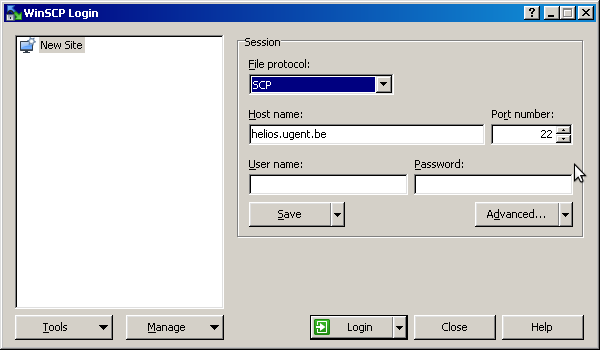
\includegraphics[scale=.5]{winscp1.png}
\end{center}
%
Hit the ``Login'' button, enter your account name and password, and you'll get something like this:
%
\begin{center}
	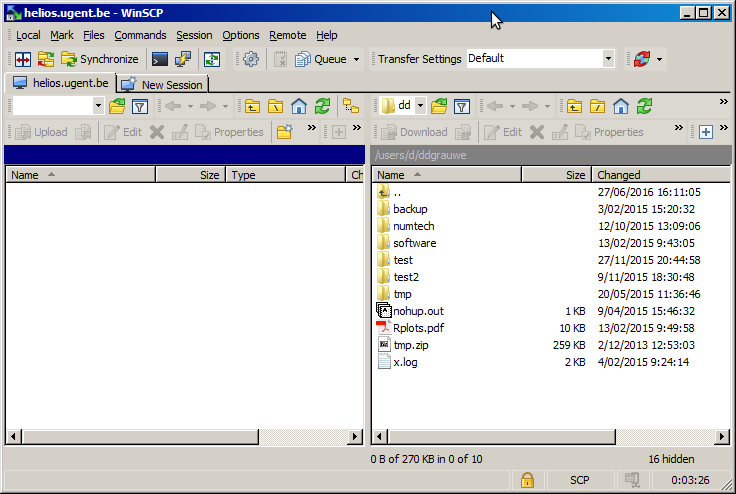
\includegraphics[scale=.5]{winscp2.png}%
	\begin{tikzpicture}
		\useasboundingbox (0,0);
		\draw [red, line width=2pt] (-12,6.85) circle [x radius=1.5,y radius=0.5];
	\end{tikzpicture}
\end{center}
%
Next, select the H-drive in the circled area of the previous screenshot, to end up with
%
\begin{center}
	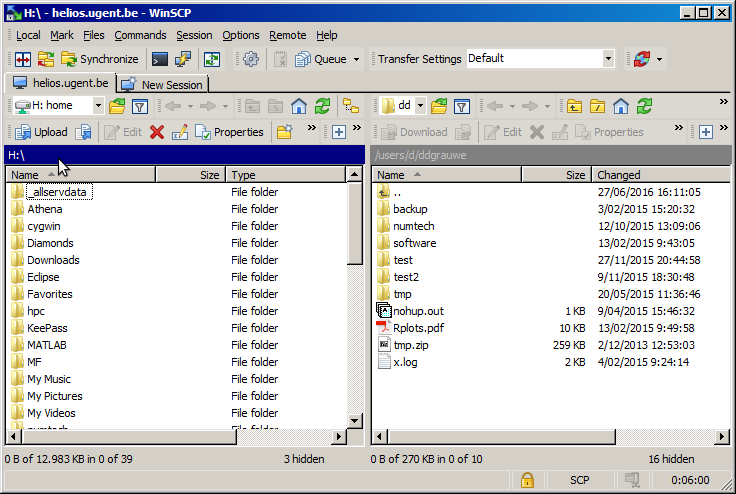
\includegraphics[scale=.5]{winscp3.png}
\end{center}
%
\par
In this window, the left panel represents your local file system (i.e. your laptop, the PC of the PC room, or the H-drive when using Athena), while the right panel represents the remote system (i.e. \texttt{helios}). Transferring files can be done by dragging between the two panels.
%
\section{Overview of programs}
%
\begin{center}
	\def\arraystretch{1.3}
	\begin{tabular}{llp{.5\textwidth}}
		Program	&	OS	&	Description	\\
	\hline
		PuTTY			&	Windows/OSX	&	make connection from Windows machine to Linux machine	\\
		Xming			&	Windows	&	enable graphical connection between Windows and Linux machine. To be used in combination with PuTTY.\\
		Notepad++	&	Windows/OSX	&	text editor	\\
		WinSCP		&	Windows		&	transfer files between two machines	\\
		RStudio		&	Windows/OSX/Linux	&	graphical interface to R; used for postprocessing and visualization	\\
		gfortran	&	OSX/Linux	&	Fortran compiler
	\end{tabular}
\end{center}
%
\end{document}
%
